\chapter{Model and backgrounds}
\label{Model_chapter}
 
\section{Signal of Interest}

The model that was studied is based on a recently proposed new mechanism of production of heavy neutrinos through the Higgs Boson decay \cite{Seesaw Mechanism with displaced vertices}. One
favourable characteristic of this model is that in a natural scenario the mass of the heavy neutrinos can lie at the electroweak scale. The theoretical study by \cite{Seesaw Mechanism with displaced vertices} 
proposes the experimental search of the heavy neutrinos using a technique known as displaced vertices.

According to this model, when the mass of the heavy neutrinos is inferior than the mass of the Higgs, the latter can present novel decay channels. The Higgs boson can decay into a light and a heavy
neutrino, followed by a subsequent decay of the heavy neutrino via a charged or neutral current interaction. Then, the decays of the heavy neutrino can be represented by: $N \rightarrow l^+ l^- \nu$
or $N \rightarrow l q q'$. Thus, there are two possible final states of the event of interest: two leptons, two jets (from the VBF process) and $\vec{E_T^{miss}}$ (due to the neutrino) or four jets 
(two of the VBF process and two from the quarks of the heavy neutrino decays), $\vec{E_T^{miss}}$ and one lepton. The first type of final state is going to be called leptonic signal, while the second
will be named hadronic signal.

If the heavy neutrino has a mass of the order of a few GeV, the Higgs and heavy neutrino would travel a certain distance before decaying. Since both particles are not detected, the decay products are expected to have associated tracks with displaced vertices. For this reason, the presence of displaced vertices in the detector is an important signal to prove this model because it could indicates the presence of the heavy neutrino in the detector. Nevertheless, in this model the resulting leptons have a low momentum. Thus, due to experimental restrictions of the available triggers in CMS and ATLAS, the theoretical analysis proposed in reference \cite{Seesaw Mechanism with displace vertices} is not achievable.  

The High Energy Physics Group at Universidad de los Andes has proposed a technique that allows to study at the LHC the production of heavy neutrinos through the decay of the Higgs boson. While in the model proposed in \cite{Seesaw Mechanism with displace vertices} considers the production of the Higgs boson through the fusion of two gluons, we consider the Higgs production through the fusion of two vector bosons. These vector bosons ($W^{\pm},Z^0,\gamma$) come from an interaction process between two quarks. Both quarks belong to protons from opposite beams that will collide in a particle accelerator. The former described process is know as Vector Boson Fusion (VBF) \cite{VBF processes}. 

Finally, as a result of the fusion of the two vector bosons, a Higgs boson is produced and the initial quarks that interacted manifest themselves as jets with high transverse momentum in opposite
hemispheres of the detector. For this reason, in Experimental Particle Collider Physics the events in which two jets of high transverse momentum are detected in opposite hemispheres of the detector 
and with a high separation of pseudorapidity are labeled as candidates of processes of VBF. The Feynman diagrams illustrating the processes already described is shown in Figure \ref{signals}, where \ref{signal_hadron_feynman} is the hadronic signal and \ref{signal_leptonic_feynman} illustrates the leptonic signal. Since it is expected that the hadronic signal have a larger cross-section than the leptonic signal, in this analysis we simulated only the hadronic signal.

%CORREGIR IMAGENEEEEEEEEEEEEEEEEEEEEEEEEEEEEEEEES

\begin{figure}[h]
\centering
\begin{subfigure}{.5\textwidth}
  \centering
  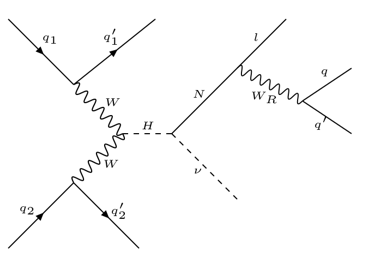
\includegraphics[width=1\linewidth]{./Capitulos/Model/hadron_signal}
  \caption{Feynman diagram for the hadronic signal}
  \label{signal_hadron_feynman}
\end{subfigure}%
\begin{subfigure}{.5\textwidth}
  \centering
  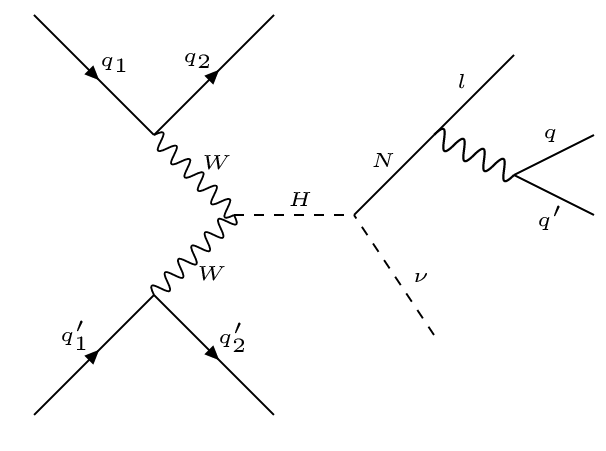
\includegraphics[width=1\linewidth]{./Capitulos/Model/leptonic_signal}
  \caption{Feynman diagram for the leptonic signal}
  \label{signal_leptonic_feynman}
\end{subfigure}
\caption{}
\label{signals}
\end{figure}


%The observation of the Higgs decay into heavy neutrinos would be a firm prove of the Type I Seesaw mechanism \cite{Type I Seesaw Mechanism}. The former would prove the existence of physics beyond the SM associated to the mass of the neutrinos.
 
 
 \section{Backgrounds}
 
The main problem of detecting an event of interest is that the magnitude of its signal is significantly smaller with respect to some other processes from the SM. For this reason, the processes from the
SM that have the same or similar final states as the signal are called backgrounds. Thus, it is fundamental to develop procedures in order to reduce the experimental background under the magnitude 
of the searched signal. These procedures usually use different variables (like the ones explain in the chapter \ref{Important_concepts_chapter}) that exploit the topology of the event and its 
kinematic characteristics. When a set of variables that separate the signal from the background is found, it is necessary to find the optimal values of them that allow to reduce as much as possible 
the background. 
 
The signal of interest that was described had two possible final states. For the hadronic signal: two leptons, two jets and $\vec{E_T^{miss}}$ and for the leptonic signal: four jets, 
$\vec{E_T^{miss}}$, and one lepton. Thus, the main backgrounds of the signal that have a similar final state are the W+jets background and the DY+jets background. In a inferior magnitude there
is other background that comes from the top pair production, referred as $t\overline{t}$.

 
\subsection{W+Jets Background}
  
%ASOCCIATEEEEEEEEEEED JEEEEEEEEEEEEEEEEETS  
The events in which is produced a W boson with jets has a large probabibity to occur in the collisions at the LHC. The W decay determines the final state of this event. The 64 \% of the times the W boson has a hadronic decay and while the rest 36\% times has a leptonic decay. In leptonic decays, the W boson desintegrates into a lepton and a neutrino. Sometimes, in these events the particles 
comming from the interaction of the initial hadrons can produce a spontaneous radiative emission, which then is detected as a jet. It is said that this kind of jet comes from an Initial State 
Radiation (ISR). Thus, when the boson W decays leptonically, the final state is conformed by a lepton, $\vec{E_T^{miss}}$ (comming from the neutrino) and jets from ISR. The Feynman diagram is shown 
in Figure \ref{w_jets_feynman}.
  
%INCLUIR FRACCIONES PRECISAS DECAIMIENTOOOOOOOOOOOOOOO
  
 \begin{figure}[h] 
 \centering
 \caption{Feynman diagram for the W+jets Background}
 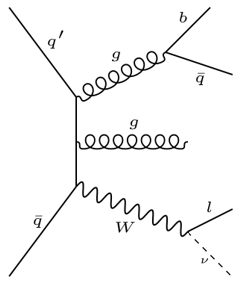
\includegraphics[width=0.4\textwidth]{./Capitulos/Model/w+jets}  
 \label{w_jets_feynman}
 \end{figure}  

 \subsection{Drell Yan + Jets Background}
 
 Other background for our signal of interest comes from the Drell Yan procces. In this process a quark and an antiquark comming from the initial interacting hadrons annihilate each other and this
 produce a virtual photon or a Z boson. The concept virtual photon means that this particle is created for a very short period of time. We studied this process only when the Z boson decays into a 
 pair lepton-antilepton, because in this case the final state is the most similar to the one of the signal. Specifically, we considered the events were the Z decays into a pair 
 tau and antitau ($\tau \overline{\tau}$). This process was simulated with the presence of a jet from ISR. Thus, the final state is conformed by one tau, jets (from the ISR procces), 
 $\vec{E_T^{miss}}$ (from the erroneus identification of the one of the taus). The Figure \ref{dy_jets_feynman} shows the Feynman diagram for this process.
 
  \begin{figure}[h] 
 \centering
 \caption{Feynman diagram for the DY+jets Background}
 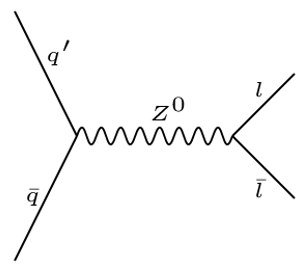
\includegraphics[width=0.4\textwidth]{./Capitulos/Model/DY+jets} 
 \label{dy_jets_feynman}
 \end{figure} 
 
 \subsection{$t \overline{t}$ Background}
 
 Other background for our signal of interest is produced by the the top anti-top creation pair. These events are produced when a gluon coming from the interaction of two colliding protons that decays into
 a pair top-antitop particles. A Feynman diagram for this background is showed in Figure \ref{t_tbar_feynman}. This figure shows that the final state of this event has three leptons, MET (coming
 from the neutrino) and one characteristic jet associated to the hadronization of a b quark. Since the signal does not have the presence of a quark b, this background can be strongly reduced by 
 making the filter of number of bjets equal to zero.
 
 %https://www-d0.fnal.gov/Run2Physics/top/top_public_web_pages/top_feynman_diagrams.html
 
  \begin{figure}[h] 
 \centering
 \caption{Feynman diagram for $t \overline{t}$ Background}
 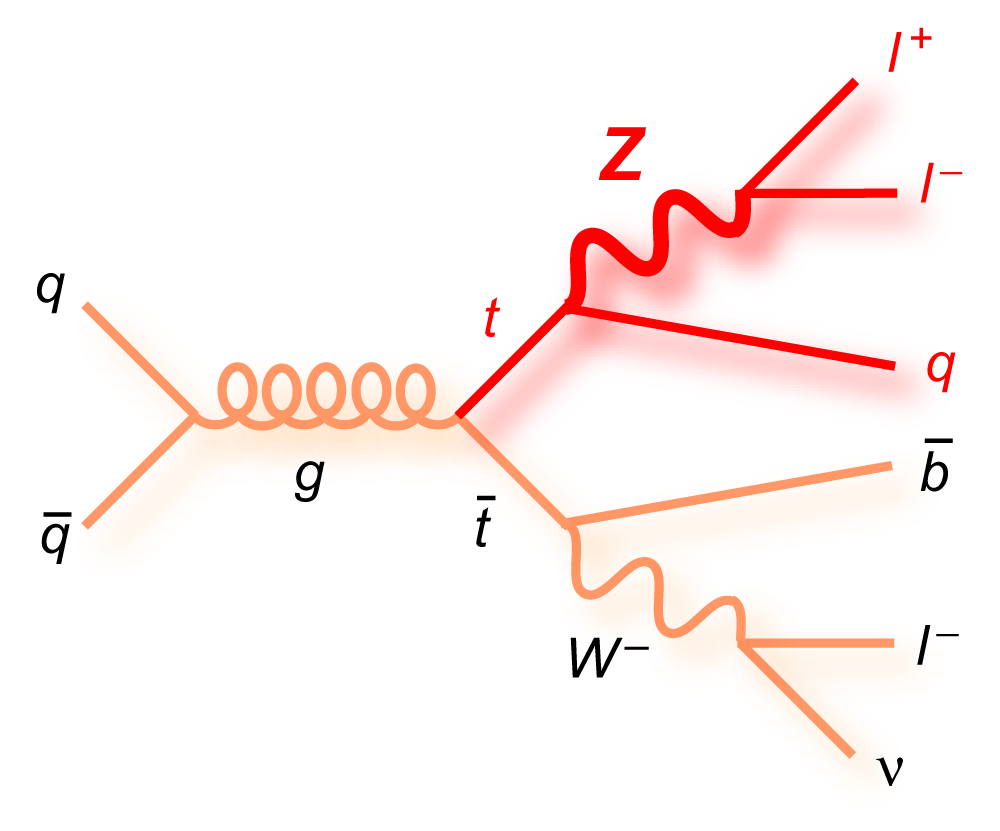
\includegraphics[width=0.4\textwidth]{./Capitulos/Model/t_tbar}  
 \label{t_tbar_feynman}
 \end{figure} 
 
 
 
 
 